%!TEX TS-program = lualatex
\documentclass[]{friggeri-cv}
\usepackage{afterpage}
\usepackage{hyperref}
\usepackage{color}
\usepackage{xcolor}
\usepackage{smartdiagram}
\usepackage{fontspec}
% if you want to add fontawesome package
% you need to compile the tex file with LuaLaTeX
% References:
%   http://texdoc.net/texmf-dist/doc/latex/fontawesome/fontawesome.pdf
%   https://www.ctan.org/tex-archive/fonts/fontawesome?lang=en
\usepackage{fontawesome}
\usepackage{metalogo}
\usepackage[utf8]{inputenc}
\usepackage{tikz}
\usetikzlibrary{mindmap,shadows}
\hypersetup{
    pdftitle={Victor Gonzalez - Software Engineer},
    pdfauthor={Victor Gonzalez},
    pdfsubject={CV Victor Gonzalez},
    pdfkeywords={cv, victor gonzalez, software engineer},
    colorlinks=false,           % no lik border color
    allbordercolors=white       % white border color for all
}
\smartdiagramset{
    bubble center node font = \footnotesize,
    bubble node font = \footnotesize,
    % specifies the minimum size of the bubble center node
    bubble center node size = 0.5cm,
    %  specifies the minimum size of the bubbles
    bubble node size = 0.5cm,
    % specifies which is the distance among the bubble center node and the other bubbles
    distance center/other bubbles = 0.3cm,
    % sets the distance from the text to the border of the bubble center node
    distance text center bubble = 0.5cm,
    % set center bubble color
    bubble center node color = pblue,
    % define the list of colors usable in the diagram
    set color list = {lightgray, materialcyan, orange, green, materialorange, materialteal, materialamber, materialindigo, materialgreen, materiallime},
    % sets the opacity at which the bubbles are shown
    bubble fill opacity = 0.6,
    % sets the opacity at which the bubble text is shown
    bubble text opacity = 0.5,
}

% \addbibresource{bibliography.bib}
\RequirePackage{xcolor}
\definecolor{pblue}{HTML}{0395DE}

\begin{document}
\header{Victor}{Gonzalez}
      {Full Stack Software Engineer}
      
% Fake text to add separator      
\fcolorbox{white}{gray}{\parbox{\dimexpr\textwidth-2\fboxsep-2\fboxrule}{%
.....
}}

% In the aside, each new line forces a line break
\begin{aside}
  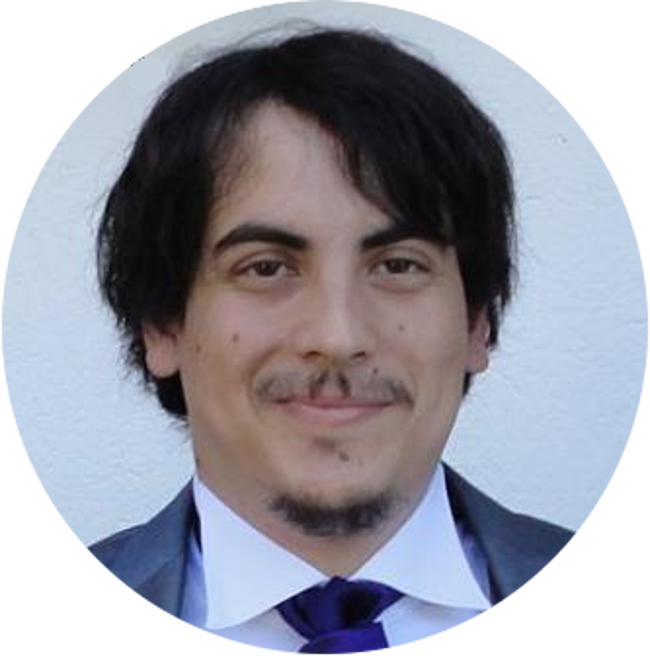
\includegraphics[scale=0.18]{img/cv_circle.png}
  \section{\faBookmark\space Personal Info}
    \textbf{Marital Status:}\\ Married
    \textbf{Home Country:}\\ Chile
    \textbf{Birthday:}\\ 27 July, 1988
    ~
  \section{\faHome\space Address}
    Las Barrancas 2581
	Apt. E203
	Quilpué
	Chile
    ~
  \section{\faPhone\space Tel \& Skype}
    \faMobile\space +56 9 8897 3537
    \faSkype\space victor.gonzalezro
    ~
  \section{\faEnvelope\space Mail}
    \href{mailto:victor.gonzalezro@gmail.com}{\textbf{victor.gonzalezro@}\\gmail.com}
    ~
  % use  \hspace{} or \vspace{} to change bubble size, if needed
  \section{Programming}
    \smartdiagram[bubble diagram]{
        \textbf{PHP},
        \textbf{Bash\vspace{3mm}},
        \textbf{Java},
        \textbf{React},
        \textbf{Python},
        \textbf{Node.JS},
        \textbf{Docker},
        \textbf{HTML}\\\textbf{JS}
    }
    ~
  \section{Personal Skills}
    \smartdiagram[bubble diagram]{
        \textbf{Team}\\\textbf{Player},
        \textbf{Initiative},
        \textbf{Always}\\\textbf{Learning},
        \textbf{Problem}\\\textbf{Solving},
        \textbf{Solution}\\\textbf{Architect},
        \textbf{TDD},
        \textbf{Organized}
    }
    ~
\end{aside}
~
\section{Experience}
\begin{entrylist}
  \entry
    {07/16 - Now}
    {Project Leader}
    {Topten International Services}
    {Lead the development of a new web platform, including the planning, budgeting and architecture design of the software, which included a 2 month internship in Zürich, Switzerland with the Topten Team.
    \\\textbf{Keywords:} \emph{Project Management, TDD, Software Architecture.}\\}
  \entry
    {12/14 - Now}
    {Full Stack Software Engineer}
    {Fundación Chile}
    {Development of several web platforms for private and public institutions of Chile. Mainly focused on energy efficency metrics, remote monitoring and control of electrical circuits using \emph{IoT and Big Data} solutions. These projects where developed from scratch, including the server stacks.
    \\\textbf{Keywords:} \emph{IoT, Software/Server Architecture, TDD, PHP, Python, Node.JS, Big Data.}\\}
  \entry
    {02/14 - 11/14}
    {Software Developer (Remote/Consulting)}
    {Fundación Chile}
    {Development of new reportability modules for an outdated energy efficiency platform, improving the UI/UX, and the inclusiong of Git versining.
    \\\textbf{Keywords:} \emph{PHP, Git, UI/UX}\\}
  \entry
    {03/13 - 12/13}
    {Software Development}
    {SubRed EIRL Ltd.}
    {Development of several static and dynamic pages for local businesses.
    \\\textbf{Keywords:} \emph{Jekyll, Wordpress, Drupal, Alfresco.}\\}
  \entry
    {05/12 - 05/13}
    {Academic Assistant}
    {Laboratory of Interdisciplinary Research on Astro-Engineering}
    {Maintaining and development of several software modules for the Atacama Large Millimiter Array Observatory, including the research for real time applications using distributed computing.
    \\\textbf{Keywords:} \emph{Java, C++, Qt, Python}\\}
  \entry
    {03/11 - 11/12}
    {Software Research Assistant}
    {Computer Systems Research Group}
    {Development of a project including low-level programming using bluetooth interfaces and distributed computing using a propietary framework of the European Southamerican Observatory (ESO).
    \\\textbf{Keywords:} \emph{C++, Qt, Python, Java, Distributed Computing}\\}
\end{entrylist}
\\
\section{Education}
\begin{entrylist}
  \entry
    {2007 - 2015}
    {Software and Computer Science Engineering}
    {Universidad Técnica Federico Santa María, Valparaíso}
    {5\+ years of software engineering and computer science classes, with a strong emphasis into project management, business intelligence, artificial intelligence and software architecture.\\}
\end{entrylist}

\newpage

\begin{aside}
~
~
~
  \section{\faNewspaperO\space Web \& Git}
    \href{http://lnked.in/vagonzal}{\faLinkedin\space lnked.in/vagonzal}
    \href{https://github.com/xzaero}{\faGithub\space github.com/xzaero}
    \href{https://gitlab.com/xzaero}{\faGit\space gitlab.com/xzaero}
    ~
  \section{OS Preference}
    \textbf{Ubuntu}
\includegraphics[scale=0.40]{img/5stars.png}
    \textbf{MacOS}
\includegraphics[scale=0.40]{img/5stars.png}
    \textbf{Windows}
\includegraphics[scale=0.40]{img/4stars.png}
    ~
  \section{Languages}
    \textbf{Spanish:} Native
    \textbf{English:} Professional Proficiency
    ~
  \section{English Level (CEF)}
    \textbf{Listening:} C1
    \textbf{Reading:} C2
	\textbf{Speaking:} C1
	\textbf{Writing:} C2
    ~
\end{aside}

\section{Relevant Skills}
\textbf{Software/Server Architecture}\\
\emph{Wide knowledge of cloud based solutions.}\\
For the past 3 years, I've been working deeply with several server architectures, from Virtual Machines to Amazon Web Services solutions, and the corresponding software architectures.\\
\\
\textbf{Continuous Integration/Deployment}\\
\emph{Continuously involved in fast delivery projects.}\\
I have useful knowledge about using Continuous Integration platforms like Travis and Gitlab CI.
\\
\section{Honors \& Awards}
\begin{entrylist}
  \entry
    {3/2012}
    {Most Innovative Project}
    {Software Fair, Santiago, Chile}
    {Given for the \emph{ALMA LEGO Simulator} project.\\
    Project developed with the support of the \emph{European Southamerican Observatory} (ESO).}
\end{entrylist}
\\
\section{Extracurricular Activity}
\begin{entrylist}
  \entry
    {2012}
    {Quantum Information Processing}
    {UTFSM, Valparaíso, Chile}
    {Short talks about the state-of-the-art on quantum computing.\\
    Dictated by Professor \emph{Dan Marinescu}, from the University of Central Florida, USA.}
  \entry
    {2012}
    {Cloud Computing}
    {UTFSM, Valparaíso, Chile}
    {Short talks about the state-of-the-art on cloud computing.\\
    Dictated by Professor \emph{Dan Marinescu}, from the University of Central Florida, USA.}
  \entry
    {2011}
    {ENEI-CLI}
    {Tandil, Argentina}
    {Encuentro Nacional de Estudiantes de Ingeniería, Congreso Latinoamericano de Ingeniería, International gathering of engineering students of South America.\\
    Seminar about engineering challenges for the engineer of the future in South America.}
  \entry
    {2011}
    {Encuentro Linux}
    {Puerto Montt, Chile}
    {National gathering of Linux users, Presentation about the ALMA LEGO Simulator project and the ALMA Common Software integration}
\end{entrylist}


\end{document}
